\begin{figure}[!h]
	\begin{floatrow}
	\captionsetup{width=.49\linewidth}
	\ffigbox{%
	\begin{subfigure}[t]{0.50\textwidth}
		\centering
		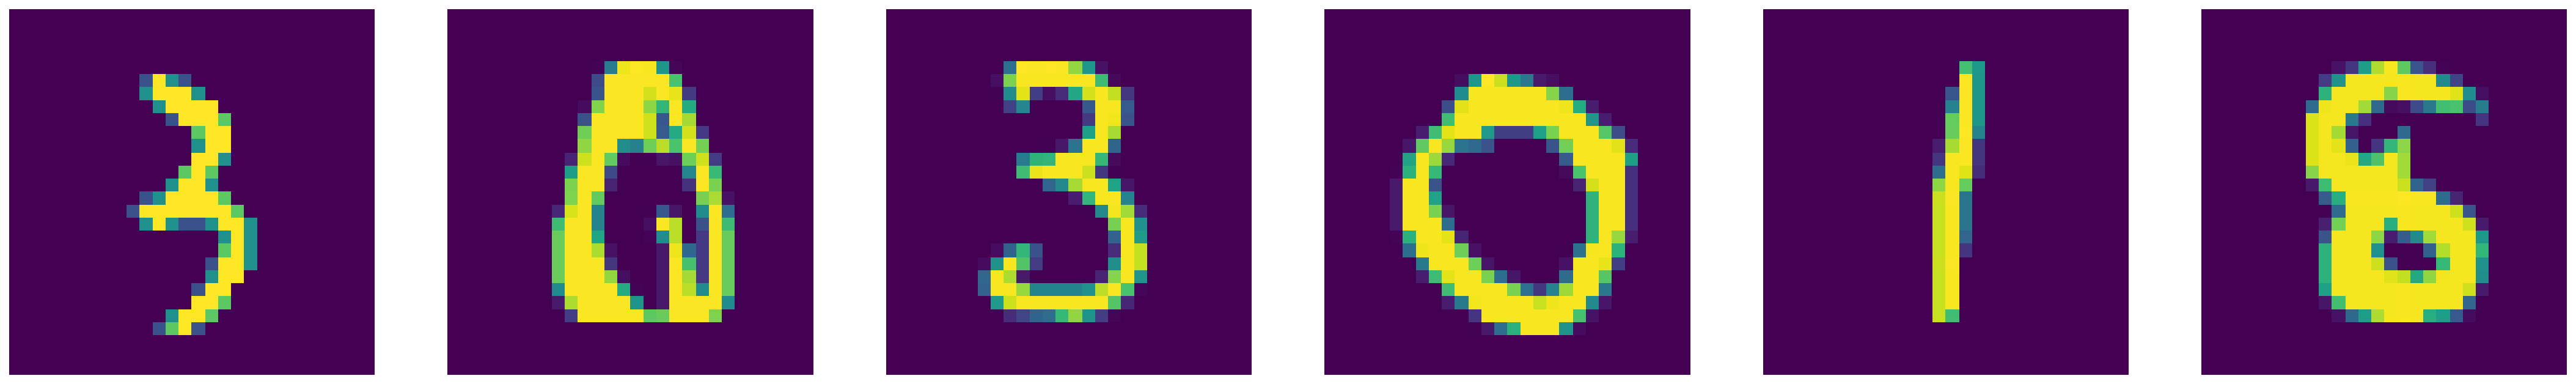
\includegraphics[width = 0.8\textwidth]{figures/ppca/real}
		\caption{Test set images}
		\label{fig:ppca:real}
	\end{subfigure}
	\begin{subfigure}[t]{0.5\textwidth}
		\centering
		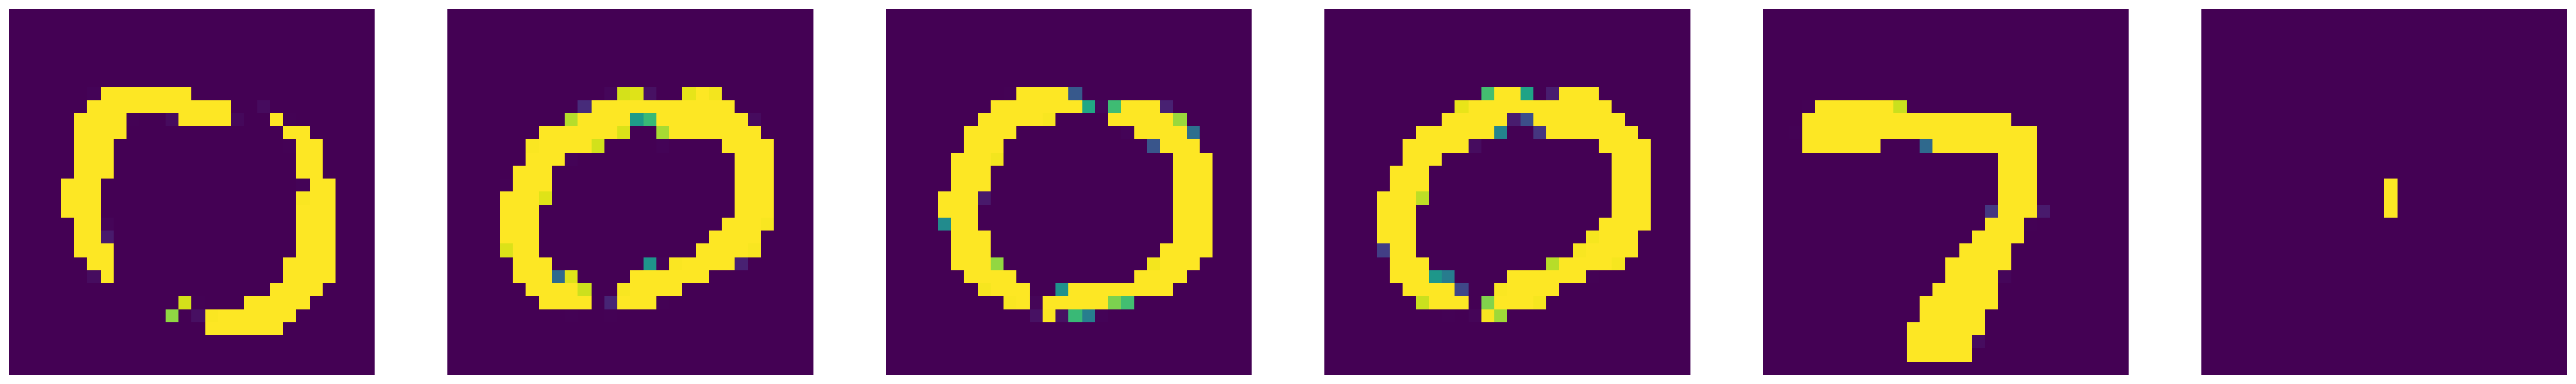
\includegraphics[width = 0.8\textwidth]{figures/vae/mean}
		\caption{VAE}
		\label{fig:vae:mean}
	\end{subfigure}
	\begin{subfigure}[t]{0.5\textwidth}
		\centering
		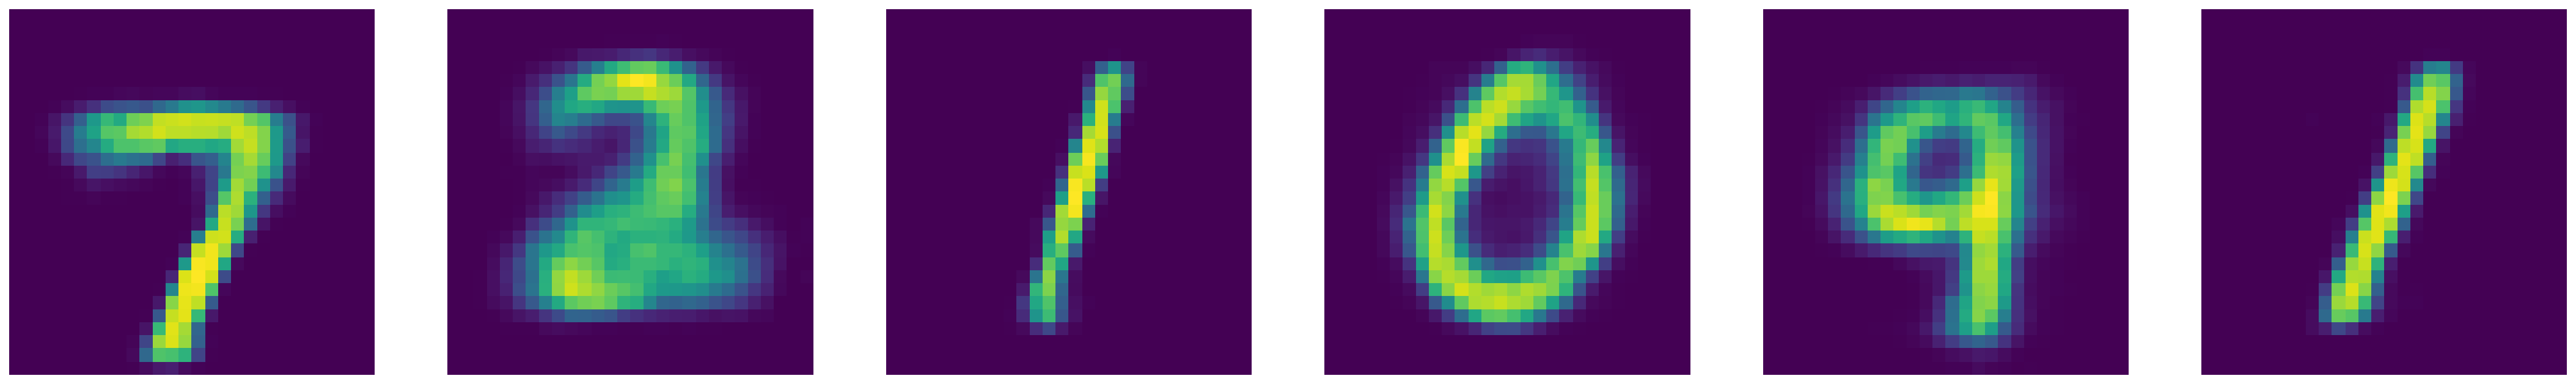
\includegraphics[width = 0.8\textwidth]{figures/cvae/mean}
		\caption{CVAE}
		\label{fig:cvae:mean}
	\end{subfigure}
	\begin{subfigure}[t]{0.5\textwidth}
		\centering
		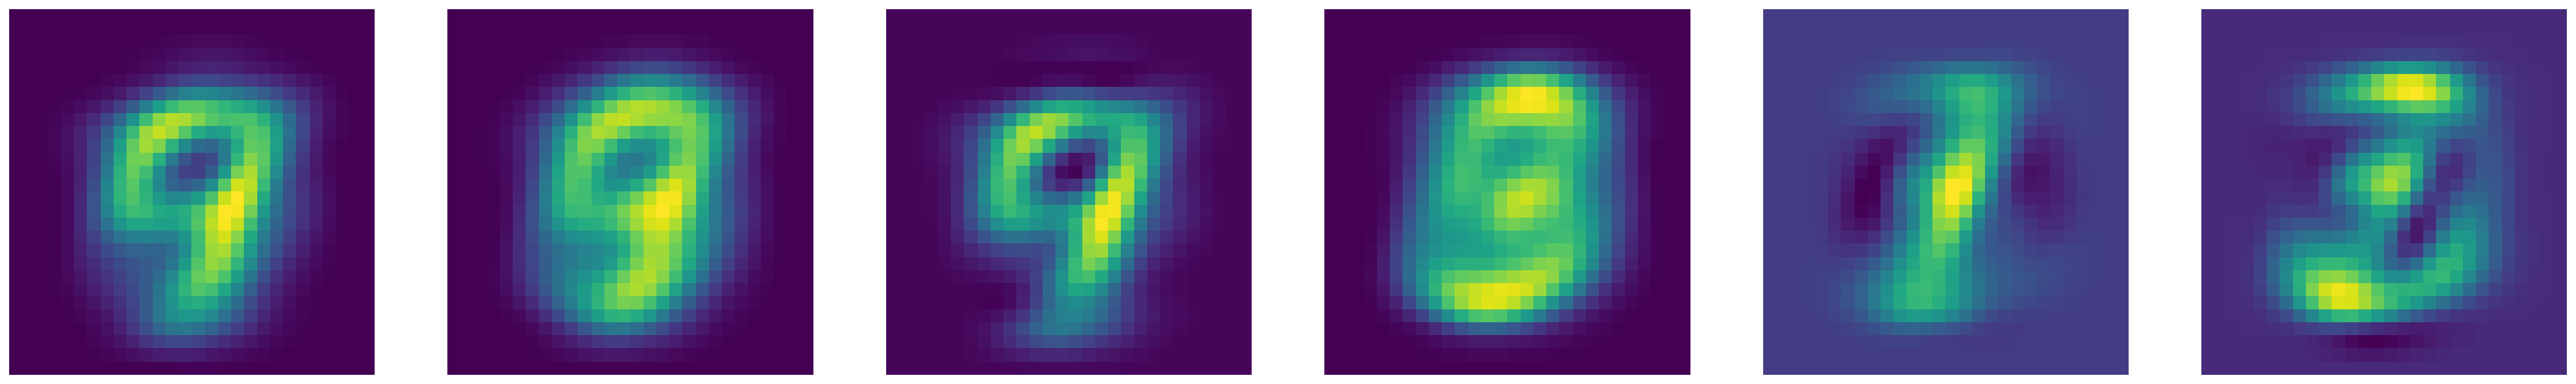
\includegraphics[width = 0.8\textwidth]{figures/ppca/mean}
		\caption{PPCA}
		\label{fig:ppca:mean}
	\end{subfigure}
	\begin{subfigure}[t]{0.5\textwidth}
		\centering
		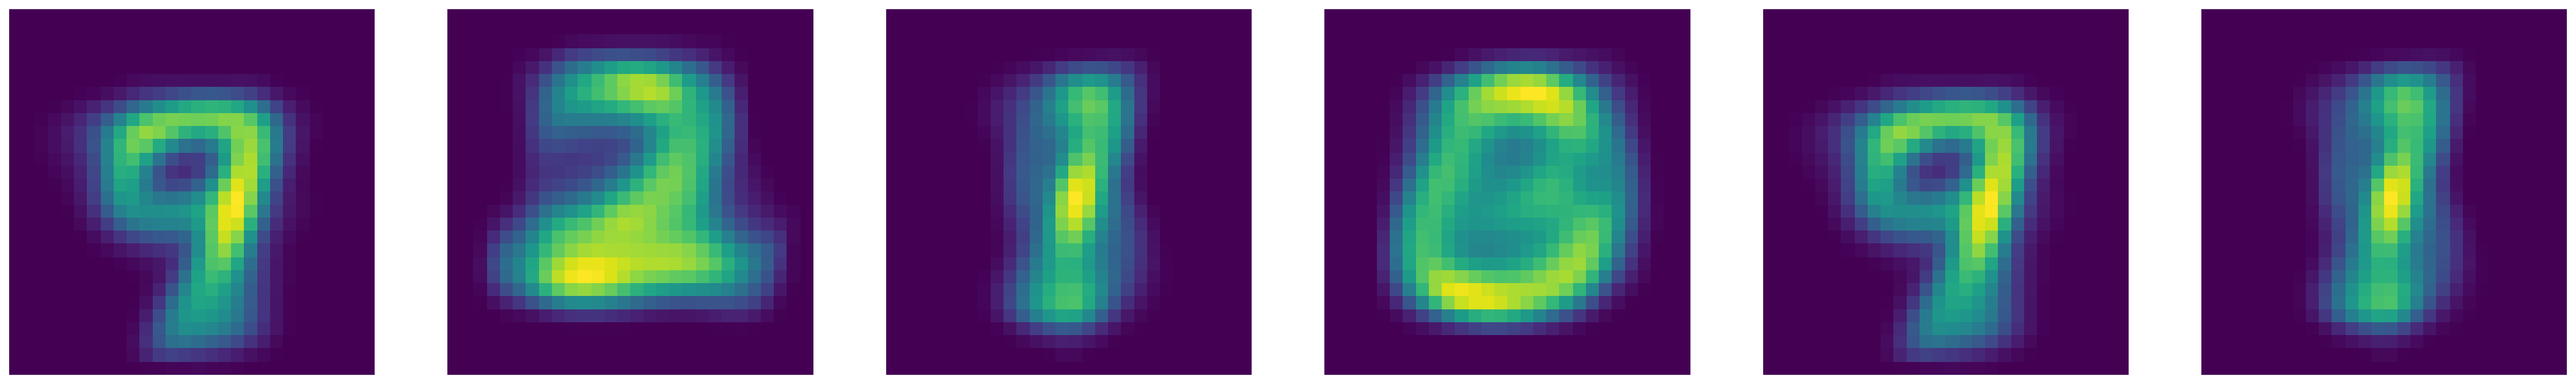
\includegraphics[width = 0.8\textwidth]{figures/gmm/mean}
		\caption{GMM}
		\label{fig:gmm:mean}
	\end{subfigure}
	
	}{%
	\caption{Comparison of MNIST test set images and corresponding mean parameters generated by density models.}
	}

	\capbtabbox{%
		\begin{tabular}{ccc}
		\toprule
		{} &  \textbf{Log-Likelihood/ELBO} &  \textbf{MSE} \\
		\midrule
		\textbf{VAE } &                 \num[round-mode=places,round-precision=4]{-1.428134e+02} &      \num[round-mode=places,round-precision=4]{0.037524} \\
		\textbf{CVAE} &                 \num[round-mode=places,round-precision=4]{-1.570527e+02} &      \num[round-mode=places,round-precision=4]{0.044375} \\
		\textbf{PPCA} &                 \num[round-mode=places,round-precision=4]{-4.329656e+03} &      \num[round-mode=places,round-precision=4]{0.055813} \\
		\textbf{GMM } &                 \num[round-mode=places,round-precision=4]{-1.066433e+07} &      \num[round-mode=places,round-precision=4]{0.058932} \\
		\bottomrule
		\end{tabular}
		
}{%
	\caption{Model performance metrics}
	\label{table:metrics}
}
	
	
\end{floatrow}
\end{figure}

\begin{figure}[!h]
	\begin{floatrow}
	\captionsetup{width=.49\linewidth}
	\ffigbox{%
	\begin{subfigure}[t]{0.45\textwidth}
		\begin{subfigure}[t]{0.49\textwidth}
			\centering
			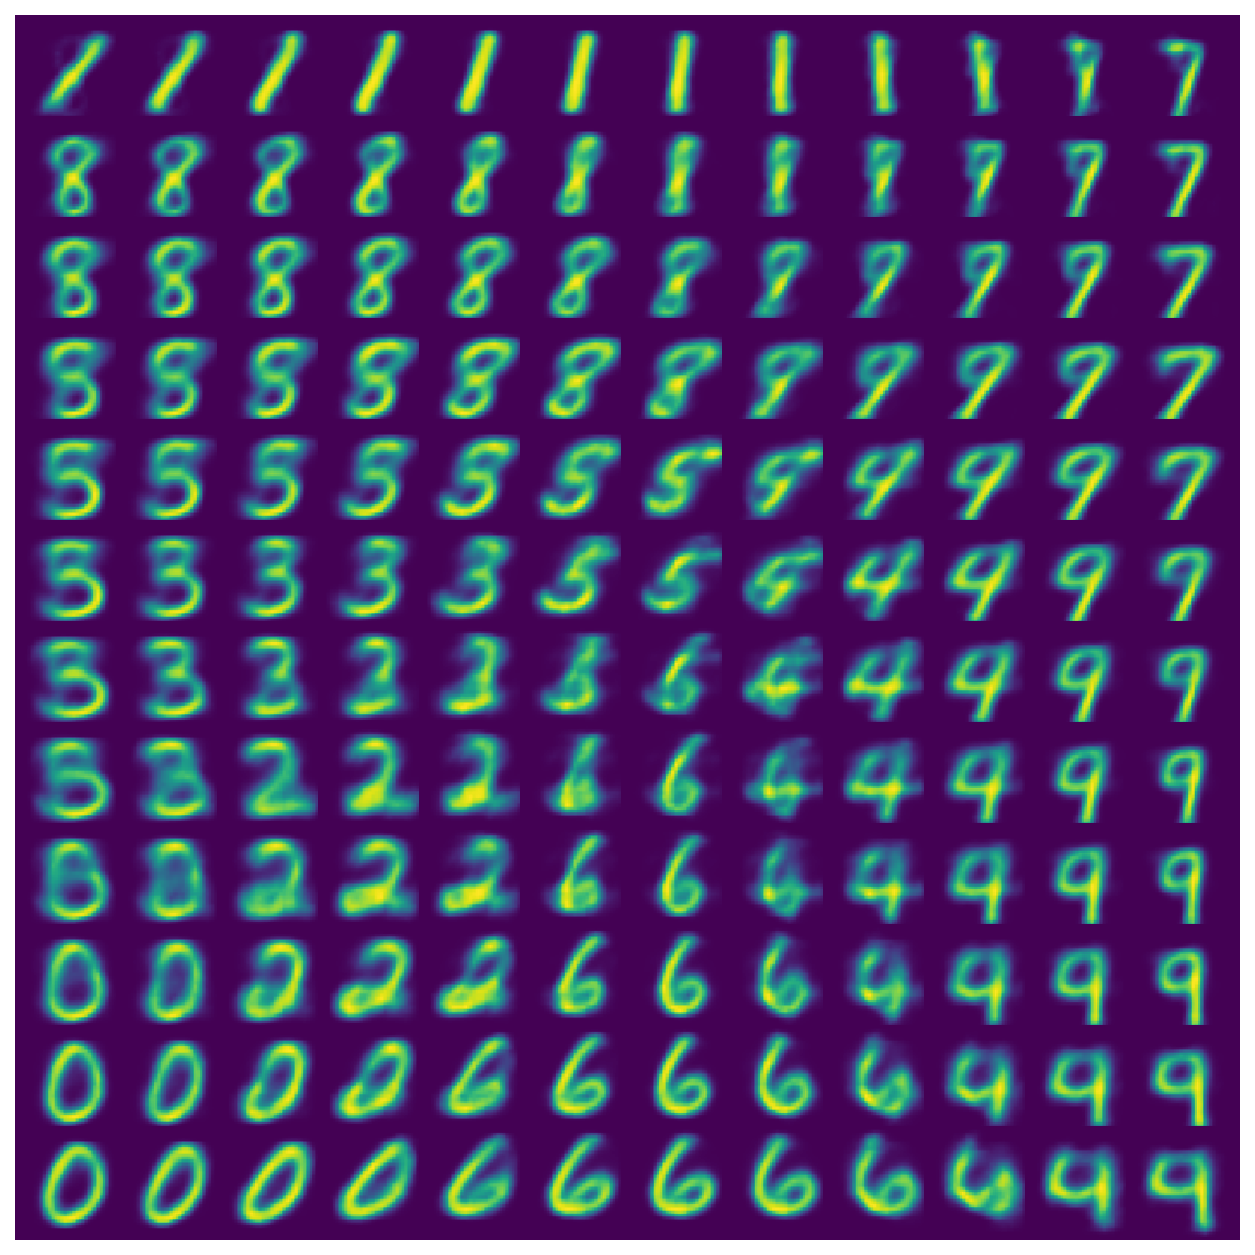
\includegraphics[width = 1\textwidth]{figures/vae/interpolation}
			\caption{VAE}
			\label{fig:vae:interpolation}
		\end{subfigure}
		\begin{subfigure}[t]{0.49\textwidth}
			\centering
			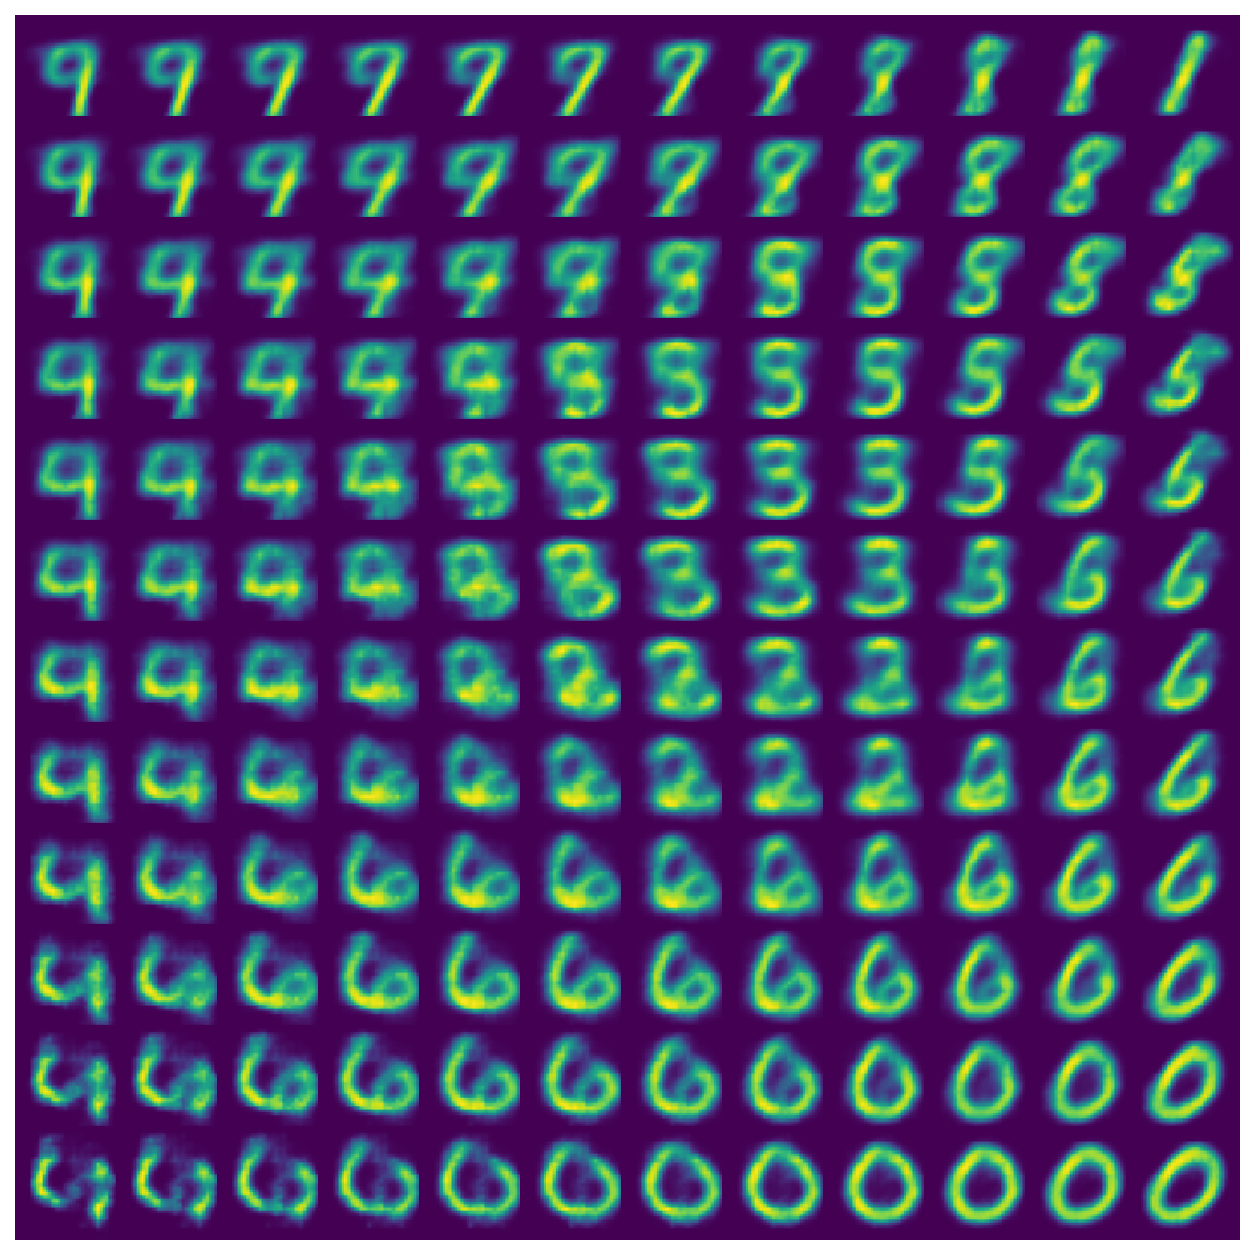
\includegraphics[width = 1\textwidth]{figures/cvae/interpolation}
			\caption{CVAE}
			\label{fig:cvae:interpolation}
		\end{subfigure}
		\begin{subfigure}[t]{0.49\textwidth}
			\centering
			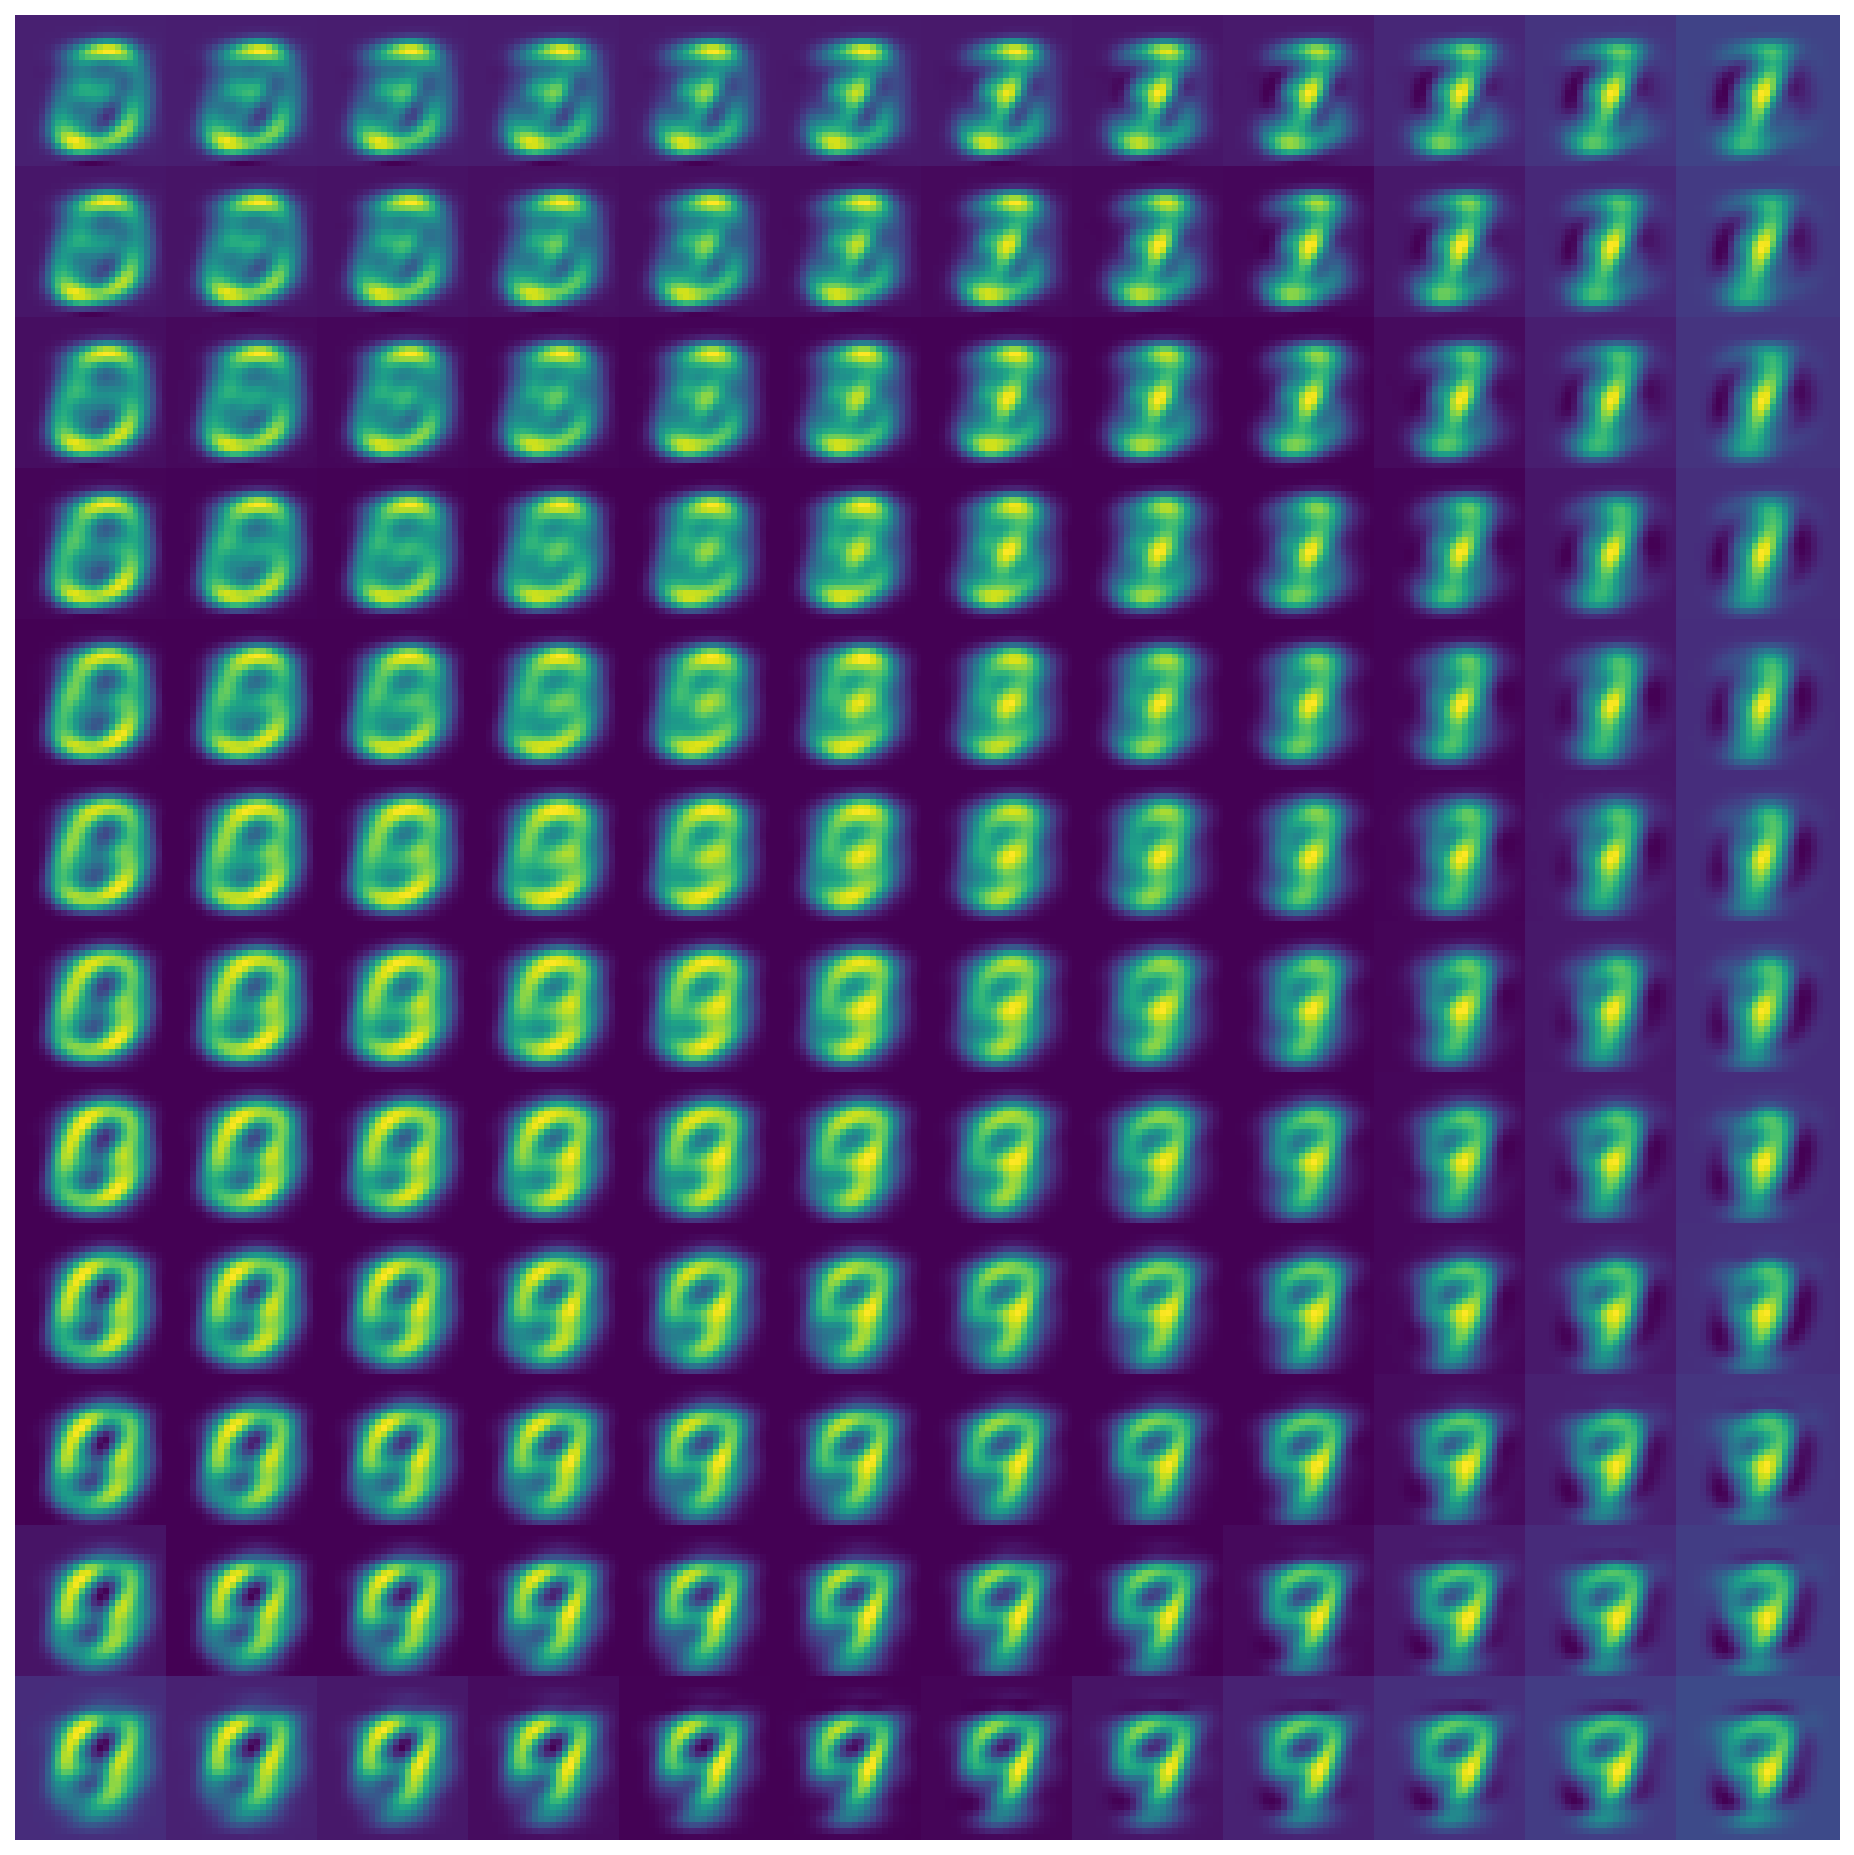
\includegraphics[width = 1\textwidth]{figures/ppca/interpolation}
			\caption{PPCA}
			\label{fig:ppca:interpolation}
		\end{subfigure}
		\begin{subfigure}[t]{0.49\textwidth}
			\centering
			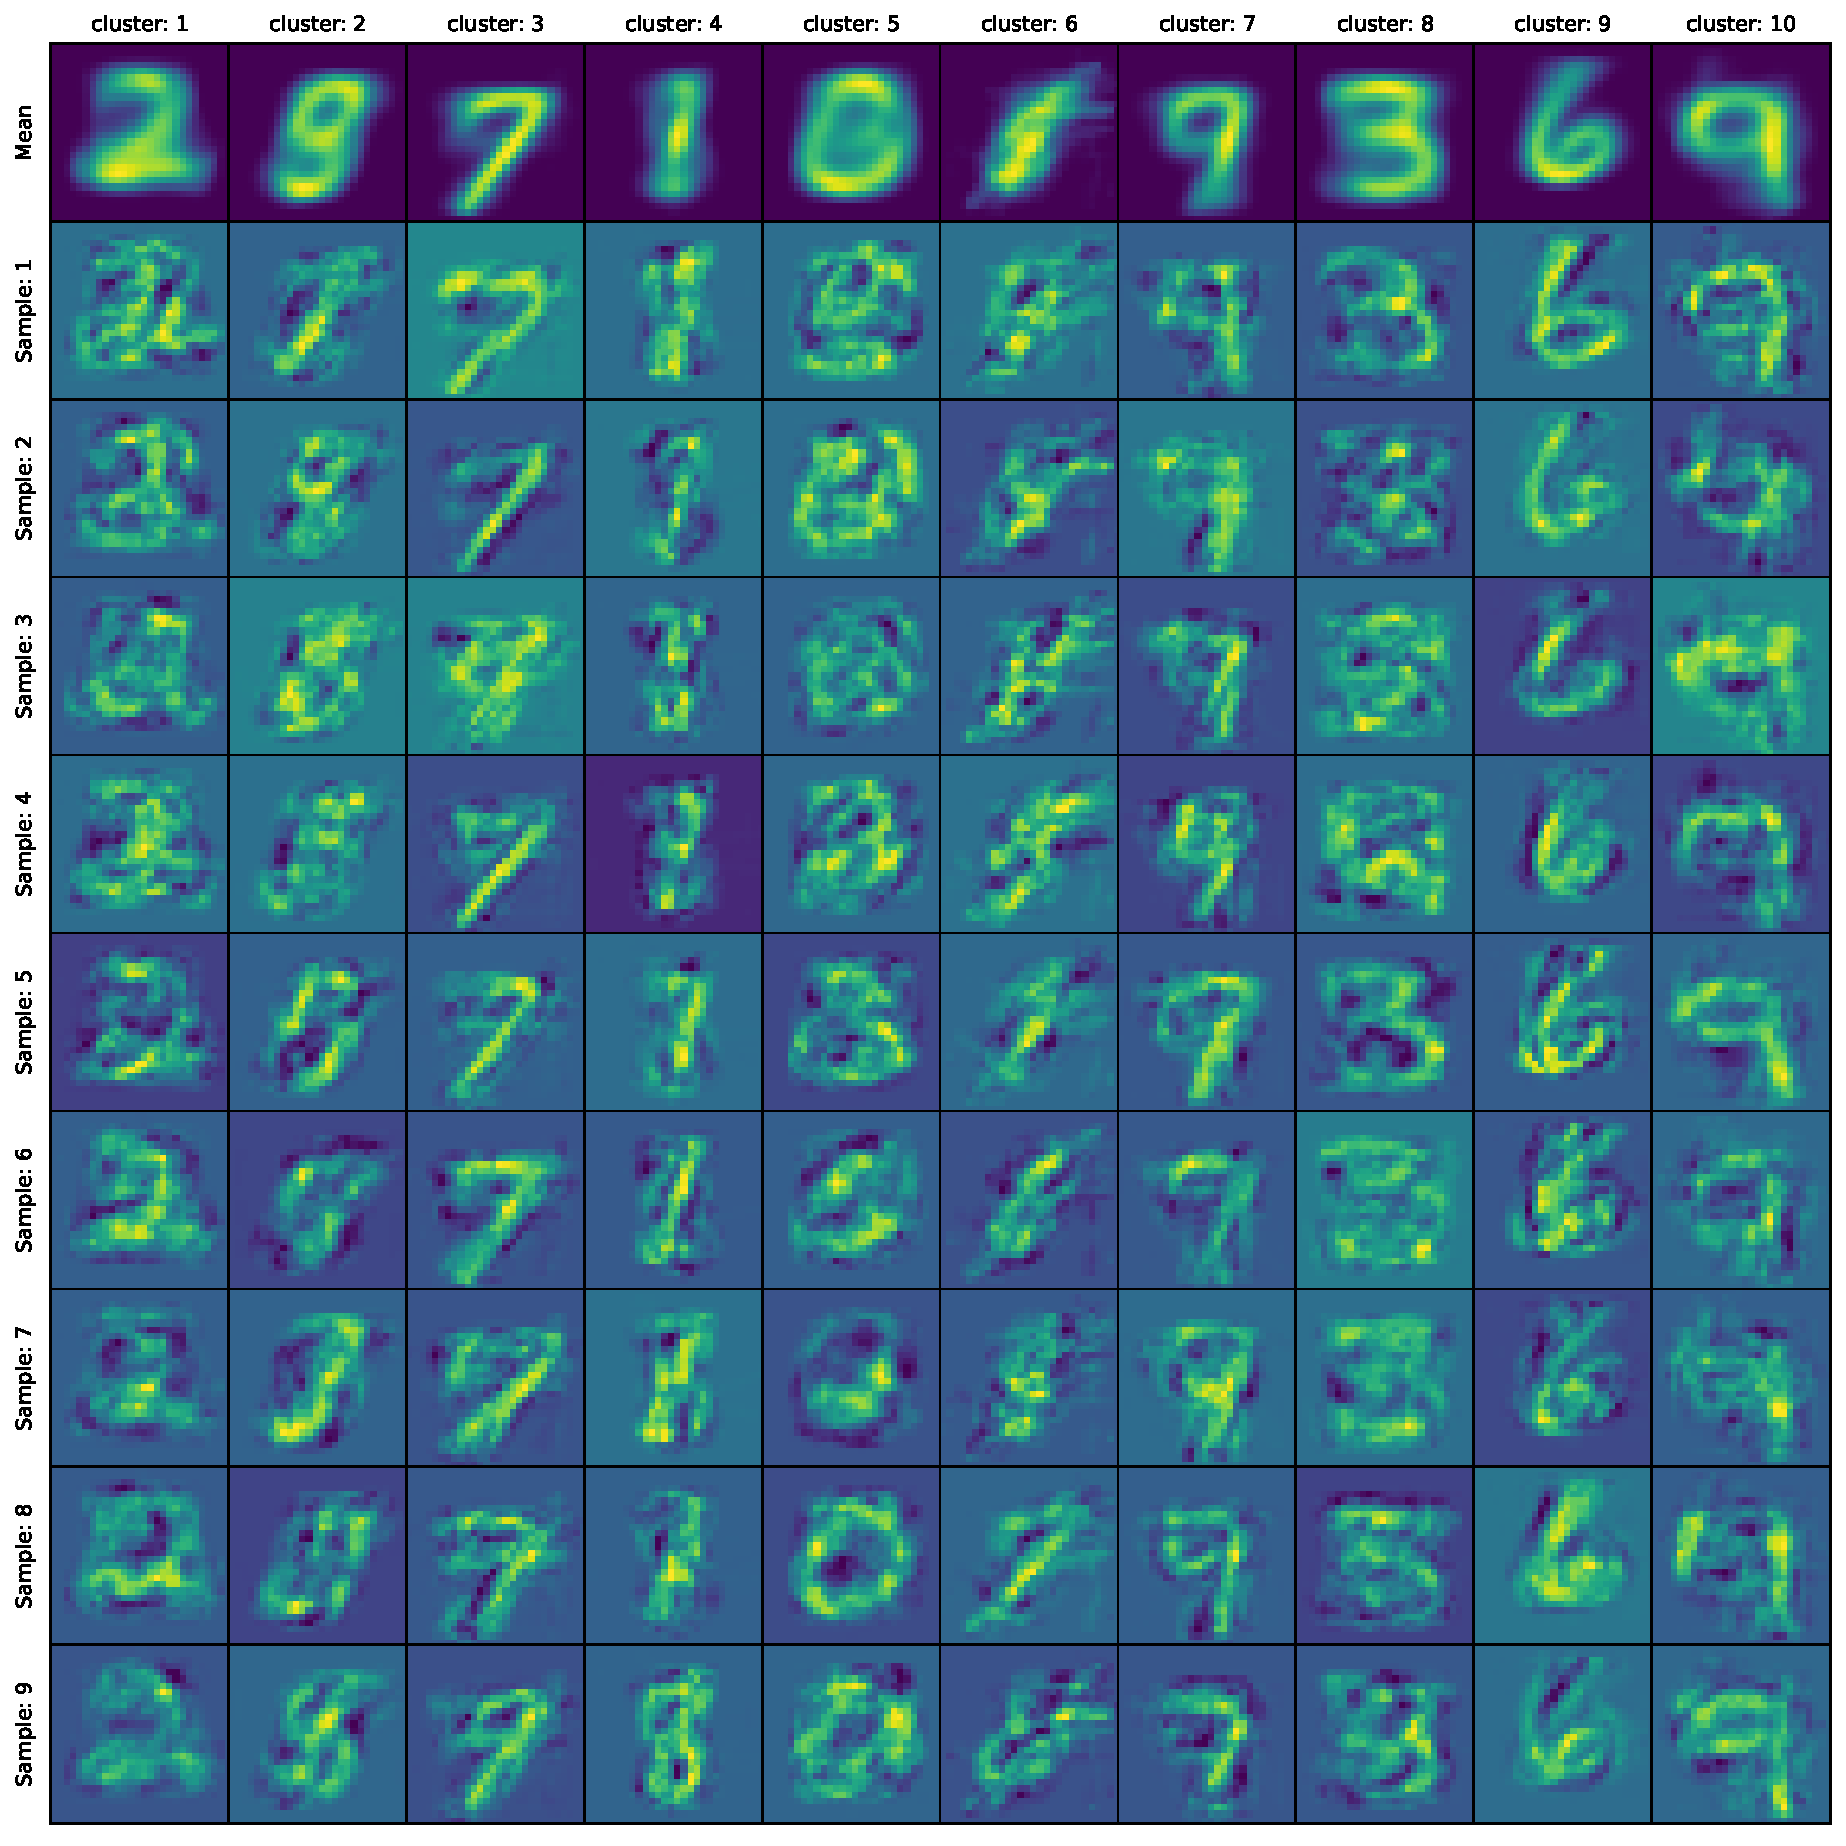
\includegraphics[width = 1\textwidth]{figures/gmm/interpolation}
			\caption{GMM}
			\label{fig:gmm:interpolation}
		\end{subfigure}	
	\end{subfigure}
	}{%
	\caption{Interpolating images from latent space variables using trained density models.}
	}
	\ffigbox{%
\begin{subfigure}[t]{0.45\textwidth}
		\begin{subfigure}[t]{0.49\textwidth}
			\centering
			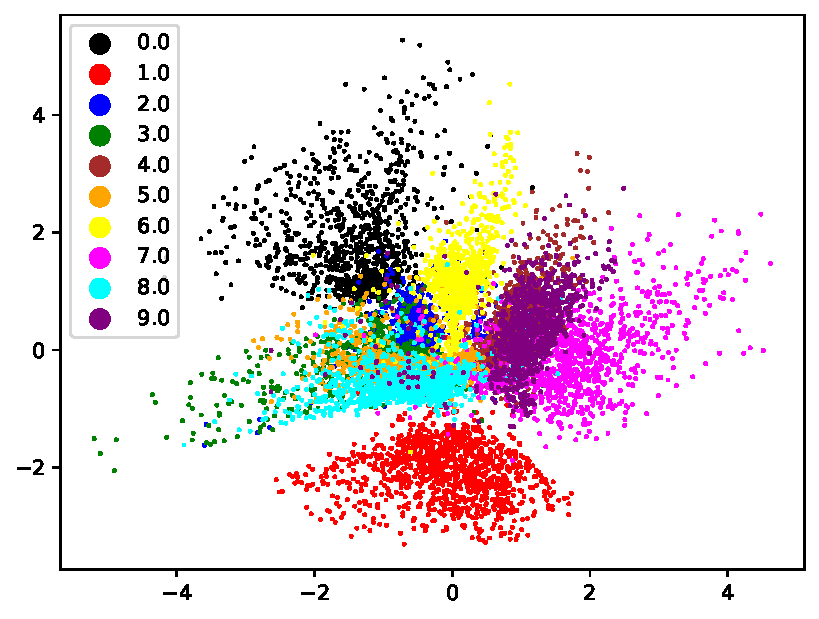
\includegraphics[width = 1\textwidth]{figures/vae/clustering}
			\caption{VAE}
			\label{fig:vae:clustering}
		\end{subfigure}
		\begin{subfigure}[t]{0.49\textwidth}
			\centering
			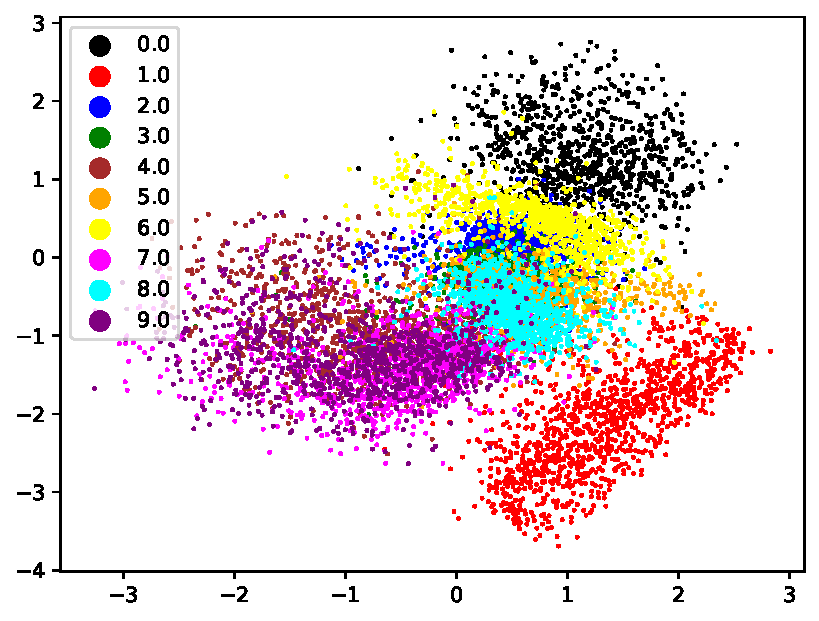
\includegraphics[width = 1\textwidth]{figures/cvae/clustering}
			\caption{CVAE}
			\label{fig:cvae:clustering}
		\end{subfigure}
		\begin{subfigure}[t]{0.49\textwidth}
			\centering
			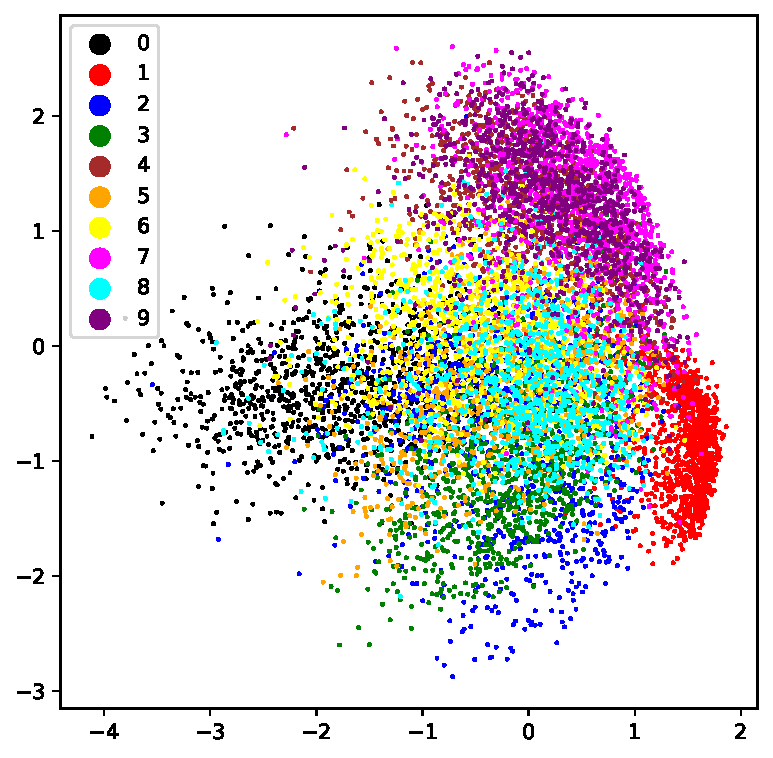
\includegraphics[width = 1\textwidth]{figures/ppca/clustering}
			\caption{PPCA}
			\label{fig:ppca:clustering}
		\end{subfigure}
		\begin{subfigure}[t]{0.49\textwidth}
			\centering
			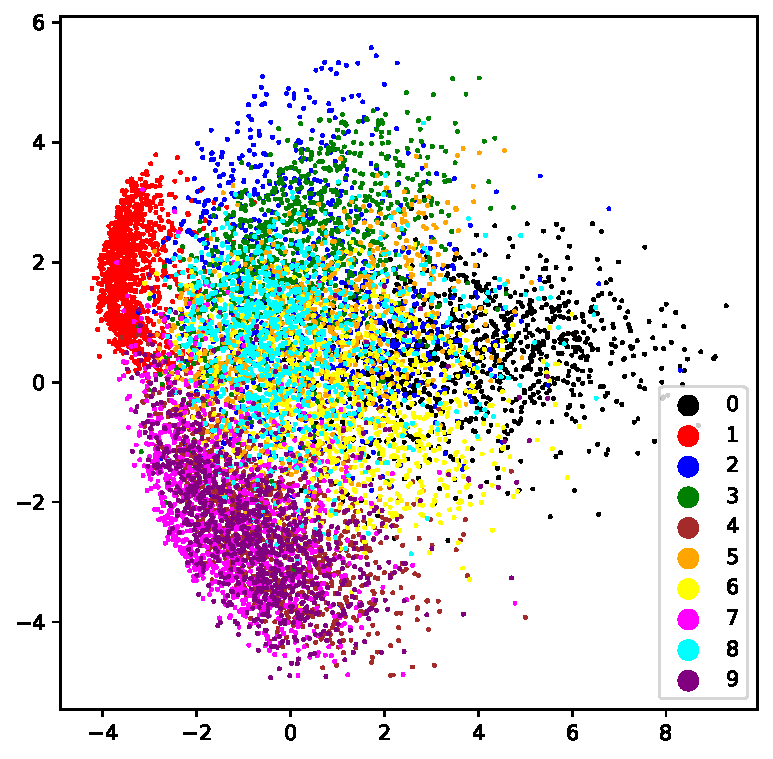
\includegraphics[width = 1\textwidth]{figures/gmm/clustering}
			\caption{GMM}
			\label{fig:gmm:clustering}
		\end{subfigure}
	\end{subfigure}
	}{%
	\caption{Clustering on MNIST test data (projection to latent space) using trained density models.}
	}
\end{floatrow}
\end{figure}

%\begin{table}
\centering
\caption{Model performance metrics}
\label{table:metrics}
\begin{tabular}{ccc}
\toprule
{} &  \textbf{Log-Likelihood/ELBO} &  \textbf{MSE} \\
\midrule
\textbf{VAE } &                   -145.122048 &      0.000305 \\
\textbf{CVAE} &                   -157.241749 &      0.000352 \\
\textbf{PPCA} &                  -4329.655559 &   3620.035365 \\
\bottomrule
\end{tabular}
\end{table}
